\section{Results}
\label{sec:results}

%This section presents the results obtained with the two background methods. 
%\subsection{The ionization method}

Figure~\ref{fig:Results_ioniz} shows the \ias\ distributions for the data and the predicted background with the background-only fits performed
by the  ionization method
in the FAIL (left) and PASS (right) regions for events passing the event selection and with \pt $>$ 200\GeV.
In the PASS region, one event is observed in the last bin (corresponding to \ias $>$ 0.4) when 0.3 $\pm$ 0.2 events are expected. 

\begin{figure}[h!]
   \centering
    \subfloat{
       \centering
       \includegraphics[width=.42\textwidth]{figures/postfit_projx2_fail_logy.pdf}
   }
    \subfloat{
       \centering
       \includegraphics[width=.42\textwidth]{figures/postfit_projx2_pass_logy.pdf}
   }
        \caption{The \ias distribution in the FAIL (left) and PASS (right) regions for events passing the the event selection and with
        \pt $>$ 200\GeV. The  data recorded in 2017 and 2018 are represented by black dots.
        The background predicted by the ionization method  is shown in yellow,
        with the hatched area indicating the background uncertainty.
       As an example, the blue line shows the 1800\GeV gluino signal distribution and the  red line shows the 557\GeV tau slepton signal distribution.
        The lower panel displays the pulls, defined as the difference between the observed (Data) and predicted (Bkg) yields divided by the associated
        uncertainty ($\sigma$).}
   \label{fig:Results_ioniz}
\end{figure}

Figure~\ref{fig:Results_mass} shows the mass spectrum for the data and the predicted background for events passing the event selection, the three special cuts on $I_h$,  
$I_{trk}^{\Delta R< 0.3}$ and  $\sigma(p_T)/p_T$ of the mass approach, and the cuts on \ias\ and \pt\ defining the signal region : \ias $>$ 0.22 and \pt $>$ 70 GeV. 
The prediction describes well the data for masses larger than 300 GeV.

\begin{figure}[h!]
   \centering
    \subfloat{
       \centering
	\includegraphics[width=.6\textwidth]{figures/UnB_v4_2017_2018_large_region999ias100_2017_2018_pull_raph.pdf}
   }
	\caption{Mass Prediction in the signal region defined by  \ias $>$ 0.22 and \pt $>$ 70 GeV.
	The  data recorded in 2017 and 2018 are represented by black dots.
        The data driven background estimate is displayed as red markers with the yellow envelope representing 
	the quadratic sum of the statistical uncertainty and the systematic uncertainty.
	Several signal scenarios are also displayed. The last bin includes the overflow.
	The lower panel shows the pull $(Data - background)/\sigma$.}
	   \label{fig:Results_mass}
\end{figure}


%%%%%%%%%%%

The two approaches show no significant excess in the data and their results are interpreted in the context of various HSCP signal models.  
The discovery potential for ionization method is expected to be higher, while
the mass method provides slightly more competitive expected
limits.
Cross section limits are placed at 95\% confidence level (CL) using a CL$_s$ approach~\cite{Junk:1999kv, READ:JPG2002} where p-values are computed with a profile likelihood technique~\cite{Cowan:2010js} that uses a lognormal model~\cite{Eadie, James} for the nuisance parameters (as detailed in Section~\ref{sec:systematics}). 

Figure~\ref{fig:massLim1} shows the expected and observed upper limits on the signal production cross-section
for the pair production of gluino R-hadrons, as a function of their mass,
along with the theoretical predictions computed at NNLO+NNLL~\cite{Borschensky_2014},
on the left for the ionization approach
and on the right for the mass method. 
%The uncertainty bands on the theoretical cross sections include the PDF uncertainty as well as the $\mu$ and $\alpha_{s}$ scale uncertainties.
This leads to the exclusion at 95\% CL of gluino R-hadrons with a mass up to 2.03 \TeV  for the ionization method and 
up to  2.13 \TeV  for the mass method. 



\begin{figure}[h!]
   \centering
    \subfloat{
       \centering
	\includegraphics[width=.42\textwidth]{figures/limits_combine_101fb_signals_gluino_v1_HSCPgluino.pdf}
   }
    \subfloat{
       \centering
	\includegraphics[width=.42\textwidth]{figures/limit_UnB_v4_gluino_SR3_raph.pdf}
   }
	\caption{Exclusion cross section limits for gluino R-hadrons 
	obtained with the ionization method on the left and with  the mass method on the right.}
   \label{fig:massLim1}
\end{figure}

The corresponding cross-section limits for the pair production of top squark R-hadrons are displayed on Fig.~\ref{fig:massLim2}.
The ionization (mass) method excludes top squarks masses below 1.40 \TeV (1.51 \TeV). 


\begin{figure}[h!]
   \centering
    \subfloat{
       \centering
	\includegraphics[width=.42\textwidth]{figures/limits_combine_101fb_signals_stop_v1_HSCPstop.pdf}
   }
    \subfloat{
       \centering
	\includegraphics[width=.42\textwidth]{figures/limit_UnB_v4_stop_SR3_raph.pdf}
   }
	\caption{Exclusion cross section limits for top squark R-hadrons 
	obtained with the ionization method on the left and with  the mass method on the right.}
   \label{fig:massLim2}
\end{figure}


In addition, the analysis is also sensitive to lepton-like HSCP candidates. Limits have been set on the two different tau slepton production models. 
Fig.~\ref{fig:massLim3} presents the limits for tau sleptons directly produced by pair. 
The theoretical cross-sections depend on the handedness of the tau sleptons in the final state, while the signal efficency is independent on it,
allowing to extract three different mass limits for the ionization method (mass method): XX \TeV (0.52 \TeV) in case of two R-handed tau sleptons, 
0.69 \TeV (0.73 \TeV) for the LL case and XX \TeV (0.81 \TeV) if all handednesses are considered.


\begin{figure}[h!]
   \centering
    \subfloat{
       \centering
	\includegraphics[width=.42\textwidth]{figures/limits_combine_101fb_signals_ppStau_ppStau.pdf}
   }
    \subfloat{
       \centering
       \includegraphics[width=.42\textwidth]{figures/limit_UnB_v4_ppStau_SR3_raph.pdf}
   }
   \caption{Exclusion cross section limits for the 
direct pair-production of tau sleptons, obtained with the ionization method (left) and the mass method (right).} 
	\label{fig:massLim3}
\end{figure}


In the context of the GMSB model, tau slepton masses are excluded  up to 0.84\TeV for  the ionization method
and up to XXX for the mass method,
as represented in Fig.~\ref{fig:massLim4}.

\begin{figure}[h!]
   \centering
    \subfloat{
       \centering
       \includegraphics[width=.42\textwidth]{figures/limits_combine_101fb_signals_gmsbStau_gmsbStau.pdf}
   }
    \subfloat{
       \centering
%	\includegraphics[width=.42\textwidth]{figures/limits_combine_101fb_signals_ppStau_ppStau.pdf}
   }
   \caption{Exclusion cross section limits for the tau slepton production within the
 {GMSB} model,
	obtained with the ionization method (left) and the mass method (right). XXX TODO: add the mass method result ! XXX } 
	\label{fig:massLim4}
\end{figure}


Figs.~\ref{fig:massLim5} and~\ref{fig:massLim6}  present the limit for Drell--Yan production of a pair of  $\tau'$ leptons, 
assuming two different electric charge schenarios, $|Q| = 1e$ and $2e$, respectively.
Drell--Yan signals with $|Q| = 1e$ and $2e$ are excluded below 
 1.31 \TeV (1.20 \TeV)  and 1.37 \TeV (1.47 \TeV) for the ionization approach (for the mass method), respectively.

\begin{figure}[h!]
   \centering
    \subfloat{
       \centering
	\includegraphics[width=.42\textwidth]{figures/limits_combine_101fb_signals_tauPrime1e_v2_HSCPTauPrime1e.pdf}
   }
    \subfloat{
       \centering
	\includegraphics[width=.42\textwidth]{figures/limit_UnB_v4_DYQ1_SR3_raph.pdf}
   }
   \caption{Exclusion cross section  limits for the {DY}-produced  $\tau'$  samples with $|Q| = 1e$
	for the ionization method (left) and the mass method (right).}
	\label{fig:massLim5}
\end{figure}

\begin{figure}[h!]
   \centering
    \subfloat{
       \centering
       \includegraphics[width=.42\textwidth]{figures/limits_combine_101fb_signals_tauPrime2e_v2_HSCPTauPrime2e.pdf}
   }
    \subfloat{
       \centering
	\includegraphics[width=.42\textwidth]{figures/limit_UnB_v4_DYQ2_SR3_raph.pdf}
   }
   \caption{Exclusion cross section  limits for the {DY}-produced  $\tau'$  samples with $|Q| = 2e$
	for the ionization method (left) and the mass method (right).}
	\label{fig:massLim6}
\end{figure}

The mass limits obtained at  $\sqrt{s}=13$\TeV for various HSCP signal models are summarized in Table~\ref{tab:MassLimits}.  
The expected limits on the mass are very similar to the observed ones. When comparing the expected values from the two methods,
they are compatible within the errors, the mass method providing slightly better limits than the ionization methed except for
the {DY}-produced  $\tau'$ with $|Q| = 1e$.

An improvement in the exclusion mass limit is obtained for all models with respect to the previous CMS publication~\cite{Khachatryan:2016sfv},
leading to the most stringent limits to-date.

\begin{table}
  \topcaption{Expected and observed mass limits obtained using 2017-2018 data for various HSCP candidate models,
 for the two background estimate methods.}
   \label{tab:MassLimits} 
  \begin{center}
  \begin{tabular}{ccccc} \hline
     Model       & \multicolumn{2}{c}{Ionization method} & \multicolumn{2}{c}{Mass method} \\
				       & Exp. (TeV) & Obs. (TeV) & Exp. (TeV)  & Obs. (TeV) \\ \hline
	  {gluino}       & 2.08 $\pm$ 0.09 & 2.03  & 2.13 $\pm$ 0.11   & 2.13    \\
	  {stop}         & 1.45 $\pm$ 0.08 & 1.40  & 1.51 $\pm$  0.10  & 1.52    \\
	  {GMSB tau slepton}    & 0.88 $\pm$ 0.07 & 0.84  & 0.87 $\pm$ 0.09 & 0.85 \\
	  {Pair-prod. RR tau slepton} & - & - & 0.52 $\pm$ 0.07  & 0.53    \\
	  {Pair-prod. LL tau slepton} & 0.73 $\pm$ 0.08 & 0.69 &  0.75 $\pm$ 0.10  & 0.64   \\
	  {Pair-prod. L/R tau slepton} & - & - & 0.82 $\pm$ 0.10  & 0.84   \\
	  {$\tau'$ ($Q=1e$) from DY prod.}        & 1.36 $\pm$ 0.10 & 1.31  &  1.18  $\pm$  0.12  &  1.20 \\
	  {$\tau'$ ($Q=2e$) from DY prod.}        & 1.44 $\pm$ 0.17 & 1.37  &  1.46  $\pm$  0.13  &  1.47 \\
	  {$Z'_{\psi} \rightarrow \tau' \tau'$ }  & 4.01 $\pm$ 0.27 & 3.88  &  4.20 $\pm$ 0.29 & 4.22  \\ 
	  {$Z'_{SSM} \rightarrow \tau' \tau'$ }   & 4.56 $\pm$ 0.28 & 4.41  & 4.75 $\pm$ 0.28 & 4.76  \\ \hline
  \end{tabular}
 \end{center}
\end{table}

% same as above but ion method has assymetric errors
%\begin{table}
%  \topcaption{Expected and observed mass limits obtained using 2017-2018 data for various HSCP candidate models,
% for the two background estimate methods.}
%  %  In the model name, 'CS' stands for charged suppressed interaction model.
%   \label{tab:MassLimits} 
%  \begin{center}
%  \begin{tabular}{ccc} \hline
%  Model                            & Expected Mass Limits & Observed Mass Limits \\ \hline
%	                           &  \multicolumn{2}{c}{Ionization method} \\
% {Gluino}  & $M>$ 2.08\twoErr{0.09}{0.09}\TeV  & $M>2.03$\TeV   \\
% {Stop}     & $M>$1.45\twoErr{0.08}{0.09}\TeV  & $M>1.40$\TeV    \\
% {GMSB Stau}        & $M>$0.88\twoErr{0.07}{0.08}\TeV & $M>0.84$\TeV     \\
% {Pair prod. Stau}   & $M>$0.73\twoErr{0.08}{0.08}\TeV & $M>0.69$\TeV \\
% {$\tau'$ ($Q=1e$) from DY prod.}        & $M>$1.36\twoErr{0.10}{0.10}\TeV & $M>1.31$\TeV  \\
% {$\tau'$ ($Q=2e$) from DY prod.}        & $M>$1.44\twoErr{0.17}{0.11}\TeV & $M>1.37$\TeV    \\
% {$Z'_{\psi}$ decaying into a pair of $\tau'$ ($Q=2e$)}        & $M>$4.01\twoErr{0.27}{0.28}\TeV   & $M>3.88$\TeV  \\ 
% {$Z'_{SSM}$ decaying into a pair of $\tau'$ ($Q=2e$)}        & $M>$4.56\twoErr{0.28}{0.31}\TeV   & $M>4.41$\TeV  \\ \hline
%	                           &  \multicolumn{2}{c}{Mass method} \\
% {Gluino}  & $M>$2.13 $\pm$ 0.11 \TeV & $M>$2.13 \TeV            \\
% {Stop}     & $M>$1.51 $\pm$  0.10 \TeV & $M>$1.51 \TeV          \\
% {Pair-produced RR Stau} & $M>$0.50 $\pm$ 0.07 \TeV & $M>$0.52 \TeV   \\
% {Pair-produced LL Stau} & $M>$0.76 $\pm$ 0.08 \TeV & $M>$0.73 \TeV  \\
% {Pair-produced L/R Stau} & $M>$0.81 $\pm$ 0.10 \TeV & $M>$0.81 \TeV  \\
% {$\tau'$ ($Q=1e$) from DY prod.}  & $M>$1.17  $\pm$  0.12 \TeV & $M>$ 1.20 \TeV \\
% {$\tau'$ ($Q=2e$) from DY prod.}  & $M>$1.45  $\pm$  0.13 \TeV & $M>$ 1.47 \TeV \\ \hline
%  \end{tabular}
% \end{center}
%\end{table}



The results for double-charged \TauPrime through the $Z'$ resonant production are shown in Fig.~\ref{fig:massLimZPrimeTauPrime} as a 2D 
exclusion plot. The cross section for the \ZPrime is taken from $Z'_{\psi}$ models \cite{Accomando:2010fz}. The branching ratio of 
\ZPrime $\rightarrow$ \TauPrime \TauPrime is assumed to be 100\%. This plot displays the mass of the \ZPrime on the y-axis and the mass 
of the \TauPrime on the x-axis, and the observed cross section limit in the z-axis. The empty circles correspond to the 35 simulated mass points.
The cross section for the full plane is interpolated based on these 35 points.  Note, where the \ZPrime mass is 3000\GeV and each \TauPrime has 1400\GeV mass, 
the available momentum to the  \TauPrime is very small which makes the search less sensitive to that region, which then results in much higher exlcuded cross sections.

The black shaded region of Fig.~\ref{fig:massLimZPrimeTauPrime} (left)  corresponds to the area that is compatible with the {ATLAS} excess, while the black star corresponds to the best fit 
from Ref.~\cite{Giudice_2022}. 
As the closest mass point to the star is at $m_{\tau'}=600\GeV$, 
the expected exclusion limit for that particular $m_{\tau'}$ hypothesis is displayed  as a function of the \ZPrime  mass for the present
analysis in Fig.~\ref{fig:massLimZPrimeTauPrime} (right). 
The dashed vertical line corresponds to the the  \ZPrime  mass of the best fit from Ref.~\cite{Giudice_2022}. 
An interpretation of the ATLAS results based on the best fit from Ref.~\cite{Giudice_2022} and 
assuming an acceptance times efficiency of 1\% is also indicated on the plots, to allow a sensitivity comparison.
The interpreted observed cross section from {ATLAS} is at $1\times 10^{-2}$ pb while the expected excluded cross section based on this study 
is at $3\times 10^{-4}$ pb. 

 \begin{figure}[h!]
    \centering
    \subfloat{
    \includegraphics[height=.36\textwidth]{figures/ZPrimeVsTauPrimeExcludedObsXsection.pdf}
    }
    \subfloat{
    \includegraphics[height=.36\textwidth]{figures/limits_combine_101fb_signals_ZPrimePsi_TauAt600_ZPrime_NoTheo.pdf}
    }
    \caption{2D exclusion (left) showing the mass of the \ZPrime on the y-axis and the mass of the \TauPrime on the x-axis, and the observed cross section limit in the z-axis. 1D plot with fixed  \TauPrime mass (right) showing the exclusion limits comparing to an interpretation of the \textit{ATLAS} results. These results have been obtained with the ionization method.}
    \label{fig:massLimZPrimeTauPrime}
\end{figure}


 \begin{figure}[h!]
    \centering
    \subfloat{
    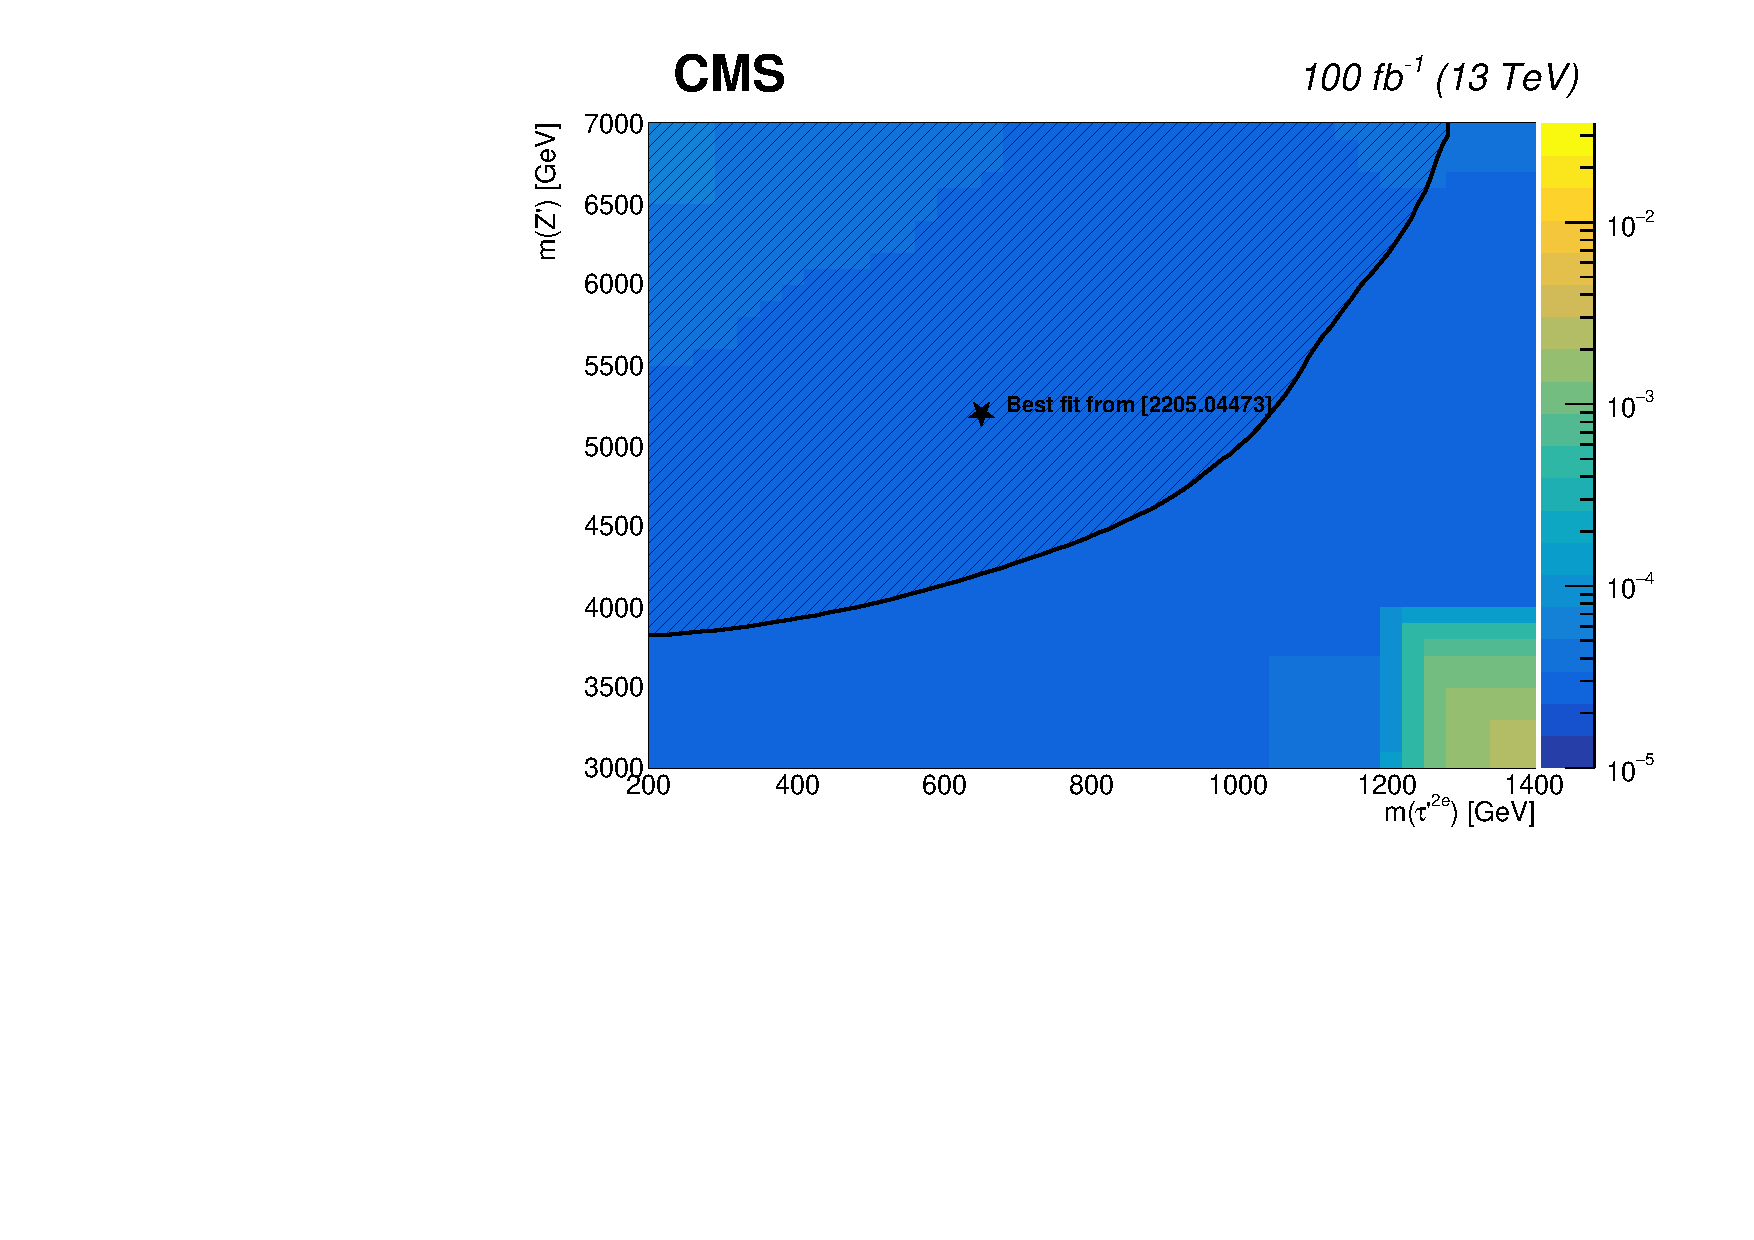
\includegraphics[height=.36\textwidth]{figures/ZPrimeVsTauPrimeExcludedObsXsection_mass_raph.pdf}
    }
    \subfloat{
    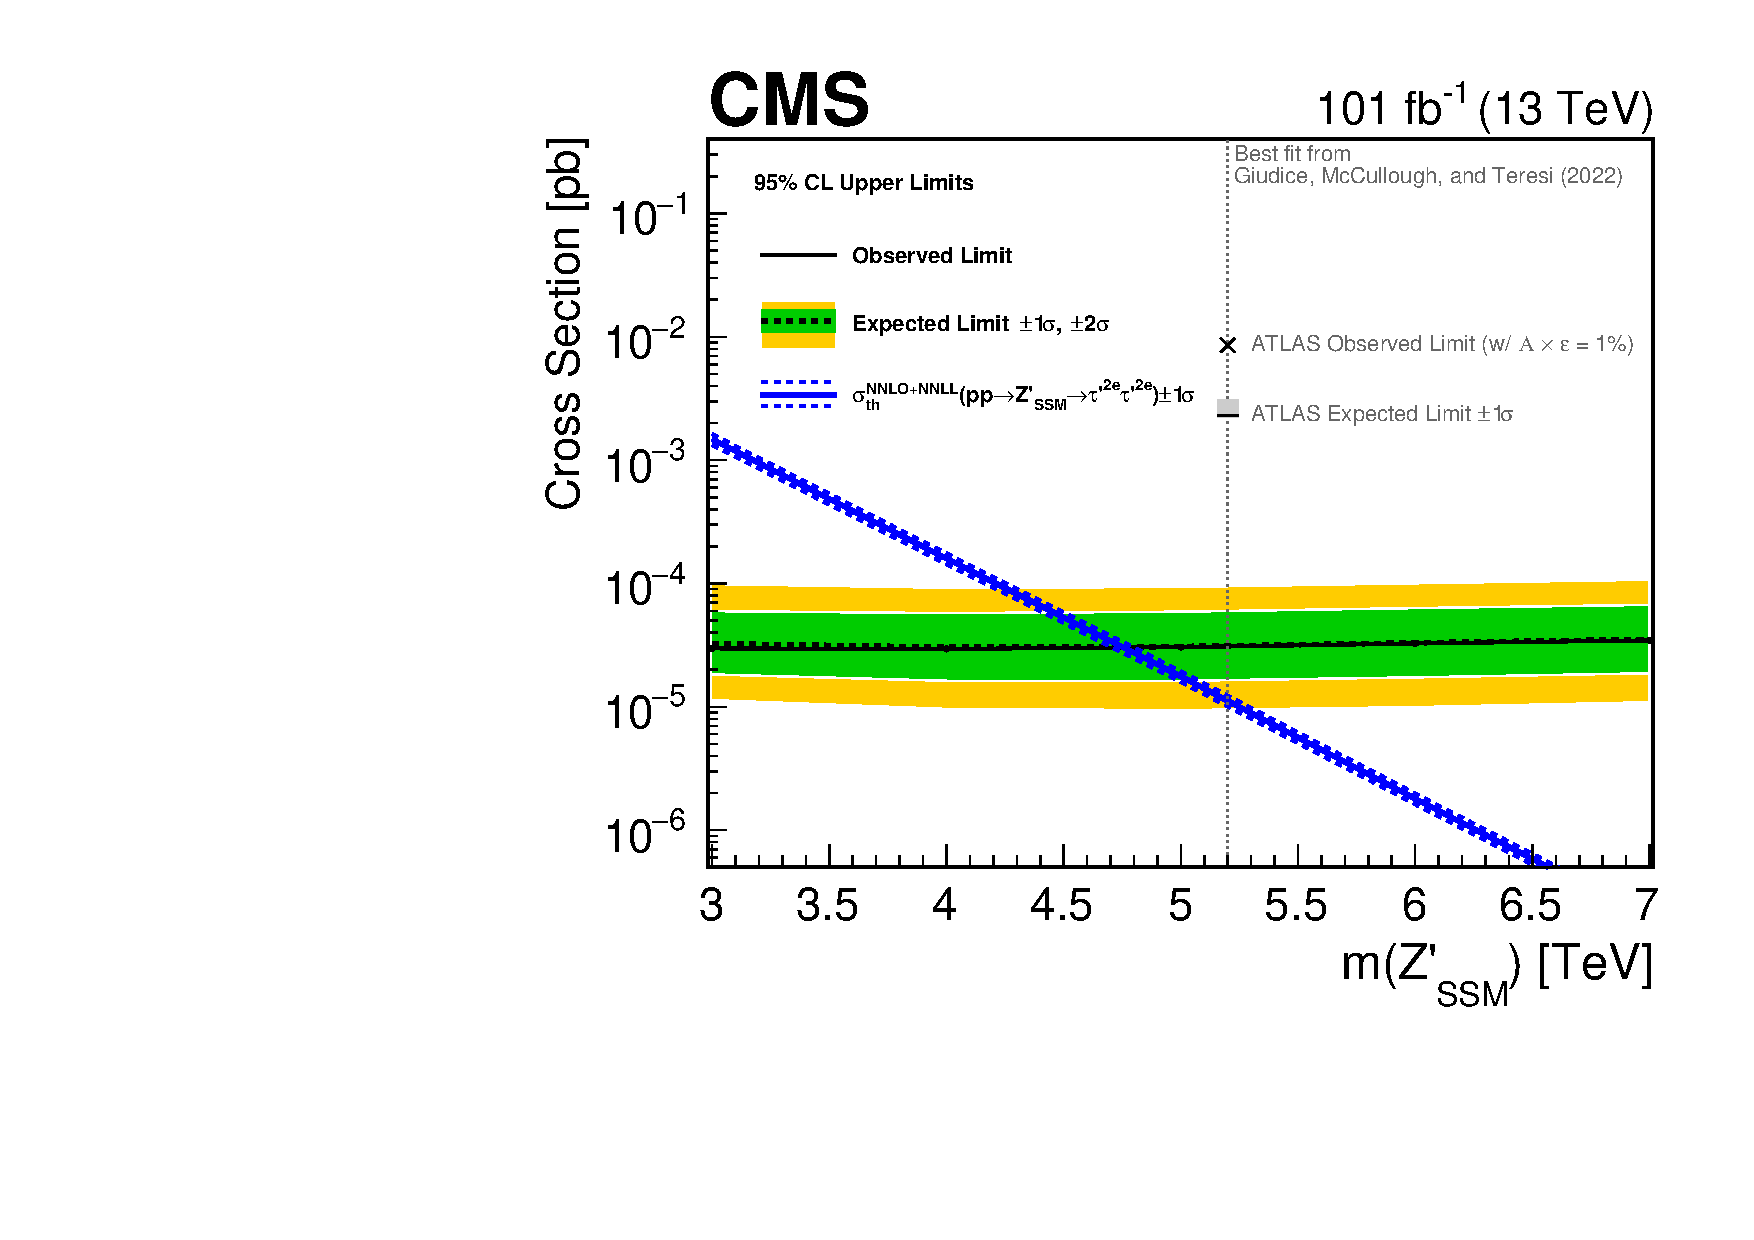
\includegraphics[height=.36\textwidth]{figures/limit_UnB_v4_ZPrimeSSM_TauAt600_SR3_NoTheo_raph.pdf}
    }
    \caption{2D exclusion (left) showing the mass of the \ZPrime on the y-axis and the mass of the \TauPrime on the x-axis, and the observed cross section limit in the z-axis. 1D plot with fixed  \TauPrime mass (right) showing the exclusion limits comparing to an interpretation of the \textit{ATLAS} results. These results have been obtained with the mass method.}
    \label{fig:massLimZPrimeTauPrime}
\end{figure}

Limits can also be set on \ZPrime models.
Figure~\ref{fig:massLimDYtauPrimeModels} shows the exclusion limits for two \ZPrime models. For the $Z'_{\psi}$ model (left) the expected mass exclusion is at 4.01\twoErr{0.27}{0.28}\TeV and the observed is at 3.88\TeV.
The same signal simulation is re-interpreted for a \ZPrime in the sequential Standard Model (SSM) theory \cite{HEWETT1989193} (right). The expected mass exclusion is at 4.56\twoErr{0.28}{0.31}\TeV and the observed is at 4.41\TeV. Since both of these are in the context of a new model, there is no direct comparison to previous results.
The improvement with respect to the $Z'_{\psi}$ model originates from the higher theoretical cross section values of the  $Z'_{SSM}$ model. The main differences between these two models are the coupling constants to the {SM} particles and the width of the \ZPrime boson. The width changes from 0.53\% in the  $Z'_{\psi}$ model to 2.9\% in the  $Z'_{SSM}$ model. The excluded cross section limit on the other hand does not change with respect to the $Z'_{\psi}$  case.

 \begin{figure}[h!]
    \centering
    \subfloat{
        \includegraphics[height=.36\textwidth]{figures/limits_combine_101fb_signals_ZPrimePsi_TauAt600_ZPrime.pdf}
    }
    \subfloat{
        \includegraphics[height=.36\textwidth]{figures/limits_combine_101fb_signals_ZPrimeSSM_TauAt600_ZPrime.pdf}
    }
    \caption{Exclusion cross section limits with fixed \TauPrime mass for the $Z'_{\psi}$ model (left) and the $Z'_{SSM}$ model (right),
	 obtained with the ionization method.}
    \label{fig:massLimDYtauPrimeModels}
\end{figure}


 \begin{figure}[h!]
    \centering
    \subfloat{
        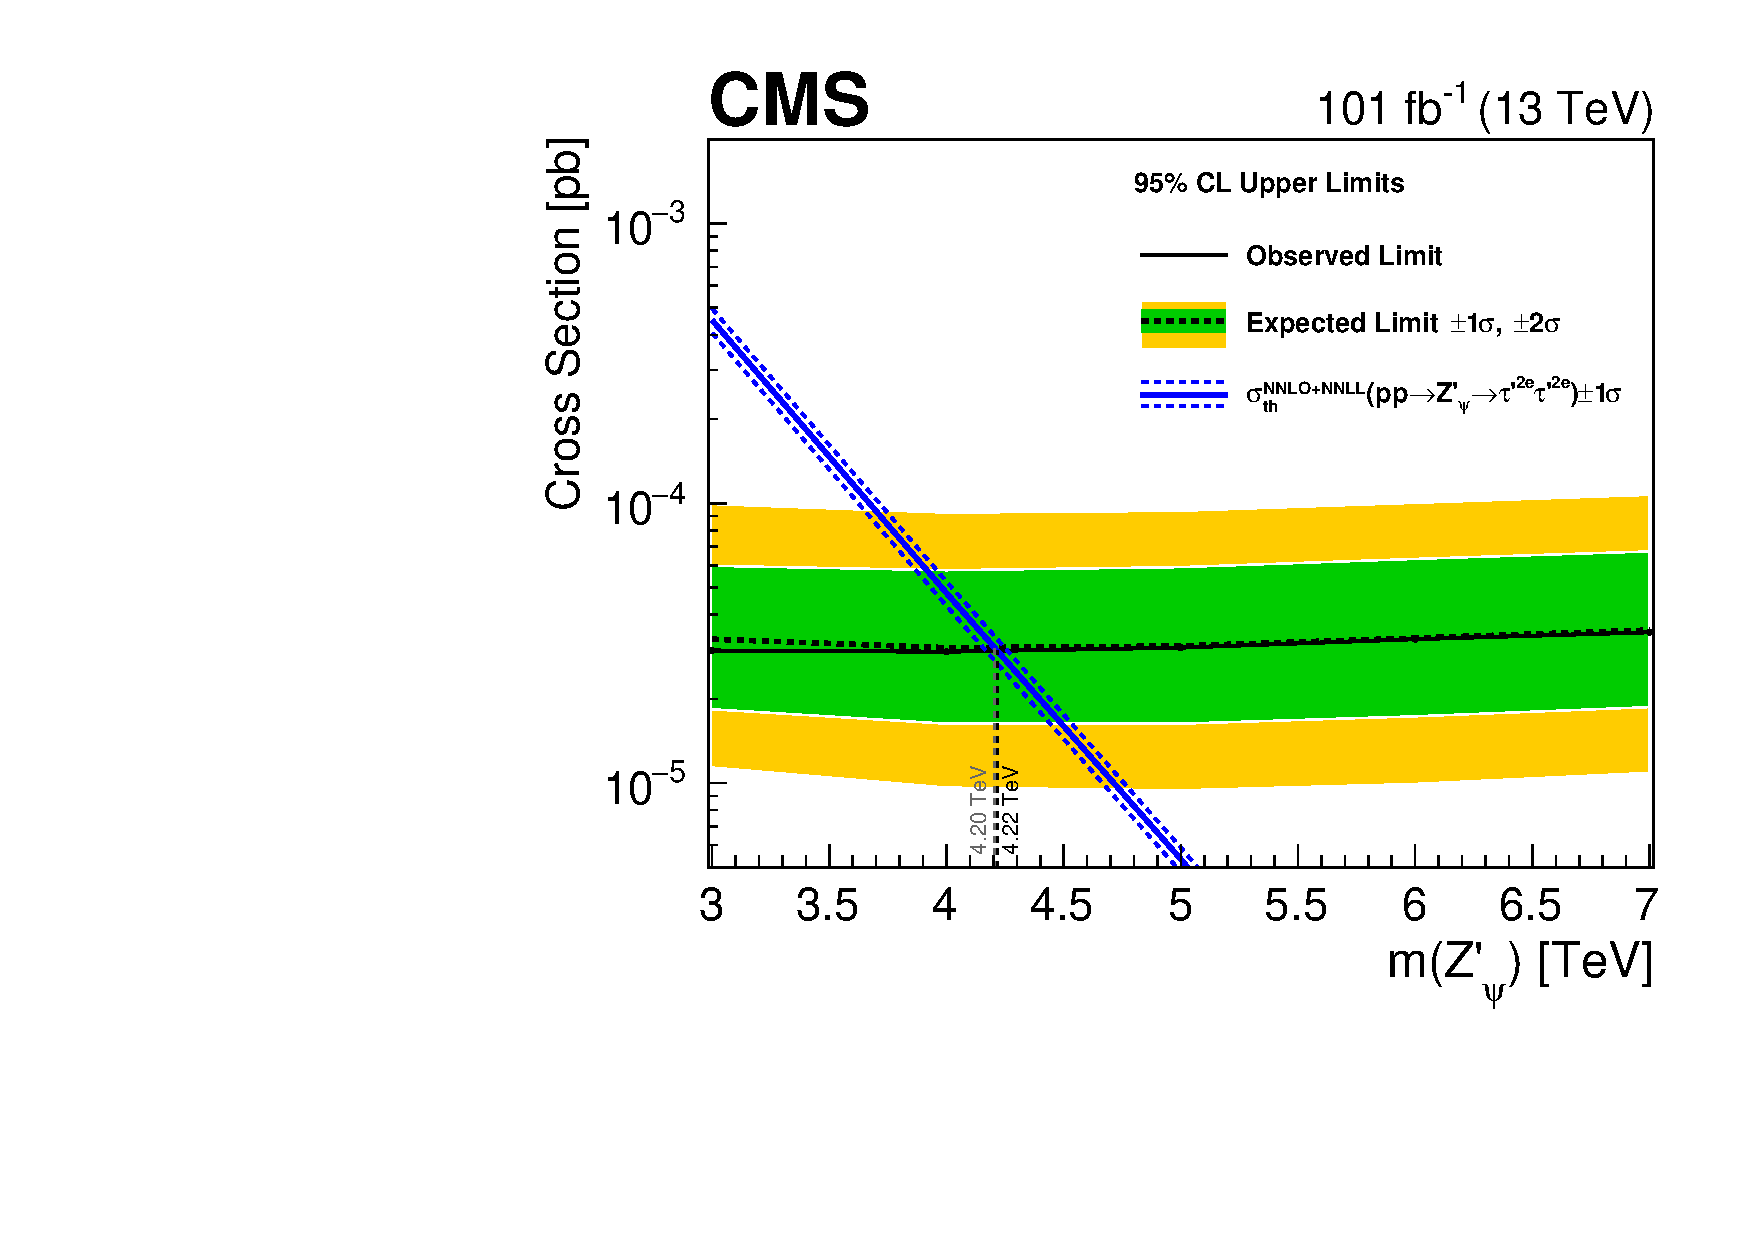
\includegraphics[height=.36\textwidth]{figures/limit_UnB_v4_ZPrimePsi_TauAt600_SR3_raph.pdf}
    }
    \subfloat{
        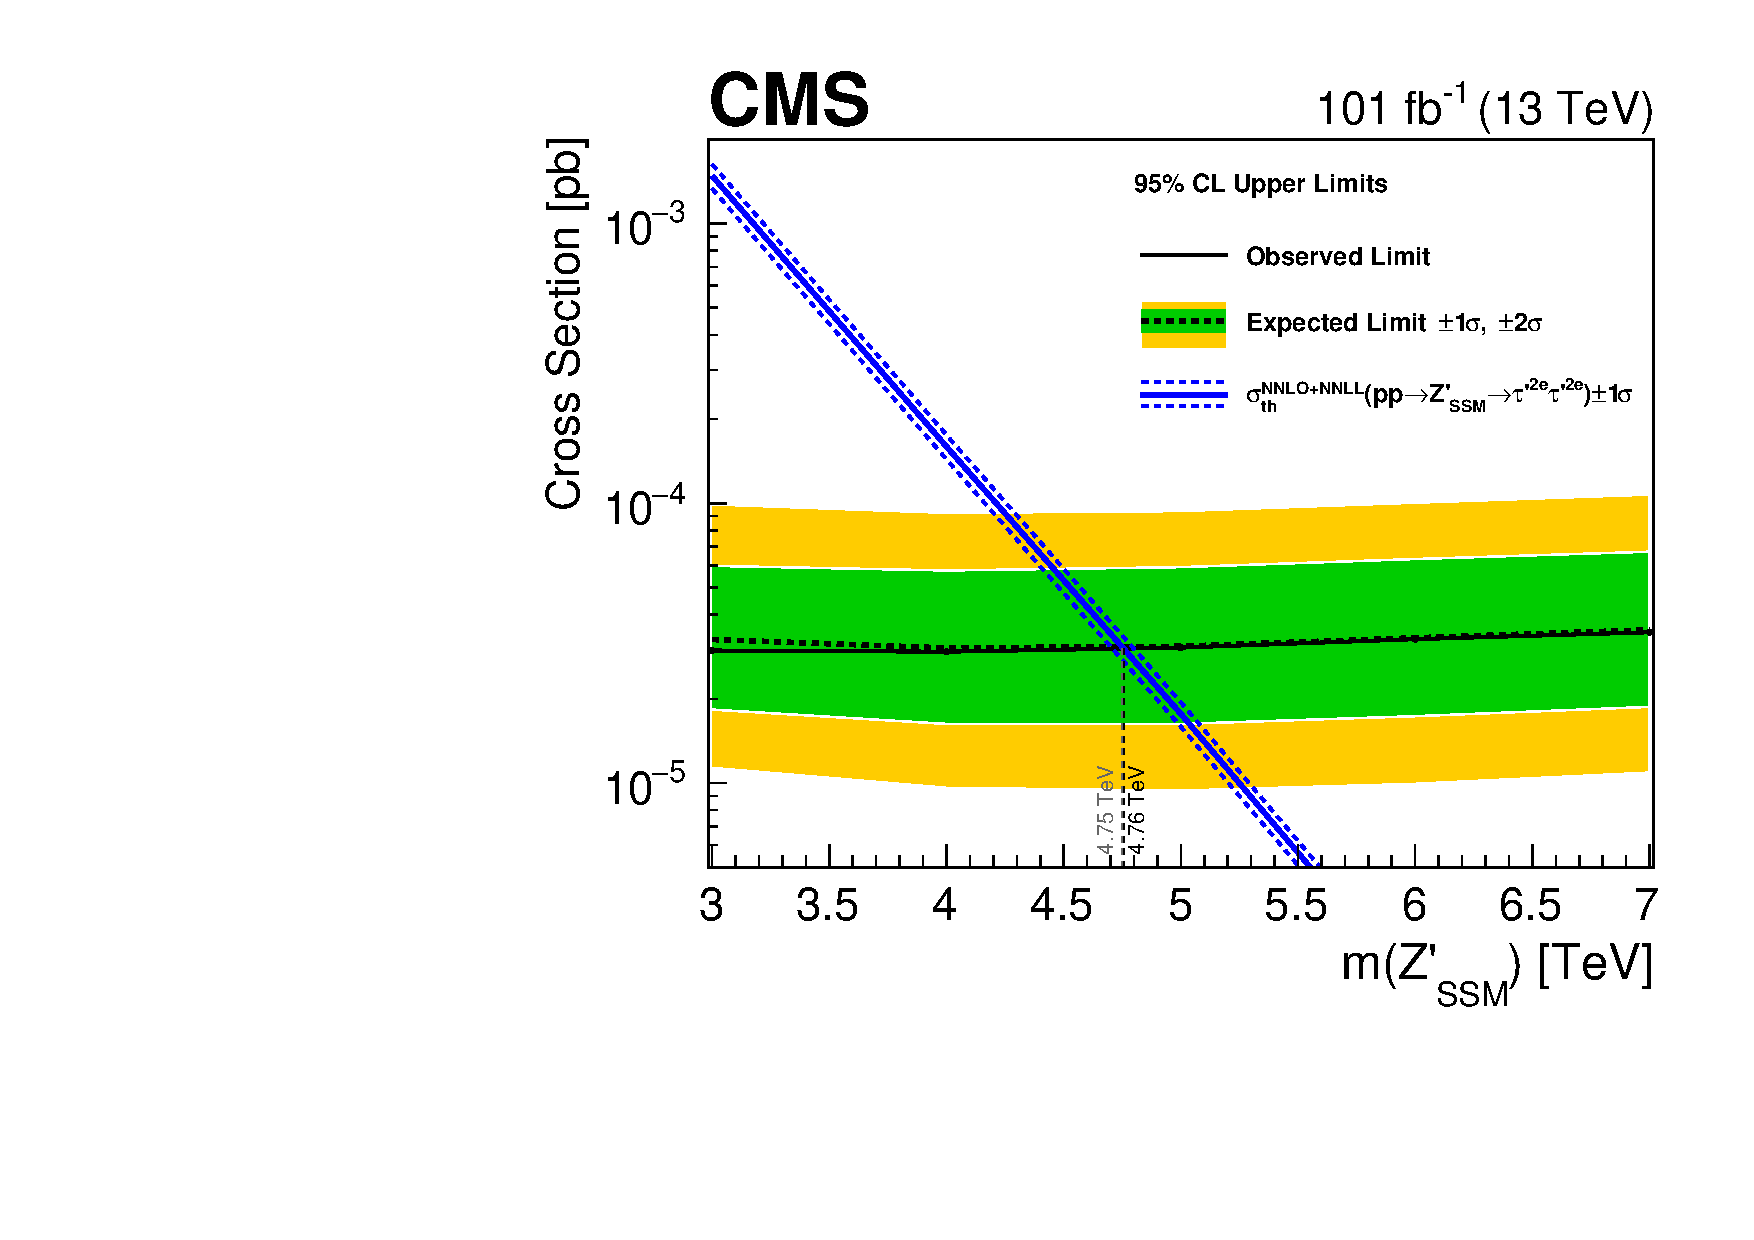
\includegraphics[height=.36\textwidth]{figures/limit_UnB_v4_ZPrimeSSM_TauAt600_SR3_raph.pdf}
    }
    \caption{Exclusion cross section limits with fixed \TauPrime mass for the $Z'_{\psi}$ model (left) and the $Z'_{SSM}$ model (right),
	 obtained with the mass method.}
    \label{fig:massLim7}
\end{figure}
